
\section{GNC Design for CubeSATs}

\subsection{Trajectory Analysis}

The trajectory of a spacecraft is crucial to the GNC subsystem. The
type of orbit that the spacecraft is designed for plays a large role
in determining the components chosen for the attitude control,
attitude estimation, and position estimation.  

There are five main trajectories that spacecrafts typically follow:
\begin{enumerate}[itemsep=-5pt]
\item LEO  (Low Earth Orbit) - Things that must be taken into account
  in this trajectory are aerodynamics, Earth albedo, and space
  debris. 
\item MEO (Medium Earth Orbit) - Van Allen Belts, which are radiation
  belts, need to be considered during the design process. 
\item GEO (Geosynchronous Orbit) - Most communication satellites are
  in geostationary orbit since the satellite appears stationary and
  the communication dishes can be pointed directly at them and do not
  need to be maneuvered to follow the satellite. 
\item HEO (High Earth Orbit or Highly Elliptical Orbit) - In this case
  you might be well outside of the GPS constellation, thus, constant
  position must be considered by an alternate means. 
\item Deep Space - A deep space orbit is largely outside of any
  protective atmosphere, therefore radiation is a dominant
  concern. Also, well beyond the GPS constellation. 
\item Propulsion, magnetorquers, and reaction wheels are the three
  main mechanisms for controlling the attitude of the
  spacecraft. Reaction wheels can be used universally, however,
  magnetorquers are only useful within a magnetic field. Thus, within
  Low Earth Orbit (LEO) magnetorquers are incredibly useful, however
  in highly elliptical orbit (HEO) they may not be nearly as
  useful. As for the third option, propulsion, it is really only
  useful outside of a magnetic field when magnetorquers are not
  ideal. A middle Earth orbit (MEO) is unique in that it can use
  everything that is offered in the LEO and HEO but it will
  continually travel through the Van Allen Belts. The Van Allen Belts
  are pockets of radiation trapped by the Earth’s magnetic field which
  require additional shielding onboard the spacecraft to mitigate its
  effects.
\end{enumerate}

In LEO, it is common to use a Global Positioning System (GPS) to
estimate the position of the spacecraft. This component is most useful
at lower altitudes because it is able to reach the GPS signal,
however, as the altitude increases and the spacecraft moves farther
away from the signal, it is no longer helpful. This is when an
integration scheme may be the best possibility for position
estimation. Integration schemes, such as RK-11, are tedious but are
commonly used in HEO. Since HEO’s have an enormous apogee compared to
perigee, up to a 35:1 ratio, the need for an alternate means to
determine position is imperative\cite{cassidis}\cite{qp2}.  

Much like a HEO, any deep space trajectory will more than likely take
the spacecraft outside of the GPS constellation. Therefore, in order
to determine position the spacecraft must use NASA’s deep space
network, a numerical analysis, or another mathematical
means. Communication with the spacecraft is another complex variable
when in a deep space trajectory. Because of the large amount of
latency between the ground and the spacecraft, the spacecraft will
need to be able to autonomously operate without a constant uplink from
the ground. Lastly, the spacecraft will need additional radiation
shielding when in deep space to protect itself. This will further
increase its mass and add further constraints to the GNC subsystem. 

Attitude estimation can be determined by the use of magnetometers,
however, similar to magnetorquers, they are only useful within a
magnetic field. Thus, magnetometers are used when the spacecraft is
set to be in LEO. There are several methods that can be used for
attitude estimation, however, the only other one that greatly depends
on the orbit are horizon sensors which must be used in LEO.

\subsection{Spacecraft Environment}

The environment of space can have an enormous impact on the spacecraft
and the GNC subsystem. The environment is dependent on the trajectory
of the spacecraft and at what altitude it is set to reach. The
environment of space changes as the spacecraft travels farther from
the earth and there can be negative repercussions depending on the
components and materials chosen for the spacecraft.  

There are four main environments that may affect a spacecraft:
\begin{enumerate}[itemsep=-5pt]
\item Earth: Does not affect the design of the spacecraft but it is
  important to keep in mind that if components are not commercial off
  the shelf (COTS), they need to be built in a lab 
\item Launch: It is crucial to research the vibration requirements
  before launching. Again, if it is not commercial off the shelf, a
  vibe test must be run to ensure the components survive.  
\item LEO: This environment has many factors that must be considered
  including effects from the sun, thermal changes, Van Allen Belts
  which account for a large amount of radiation thus radiation
  shielding must be researched for the separate components. 
\item Deep Space: There are some things such as meteorites that may
  need to be considered, however, there is not much that can be
  done. This environment should not heavily affect the design.
Note that the spacecraft is going to undergo multiple types of
disturbances as explained in the dynamic model section.
\end{enumerate}

\subsection{Spacecraft Attitude Control}

Attitude control is the means by which the orientation of the
spacecraft is maintained within the orbit. Throughout the mission, the
spacecraft experiences disturbance torques that are caused by a
variety of sources, such as aerodynamics, gravity gradient, and solar
radiation pressure discussed previously. These torques impart momentum
which rotate the system away from its desired orientation. The purpose
of attitude control is to reject these disturbance torques while
simultaneously pointing towards a desired orientation. Possible active
mechanisms for attitude control are magnetorquers, reaction wheels,
thrust vector control, reaction control system, and control moment
gyros.

There are several components that can be used for the attitude control
of a satellite. Selecting the proper component is dependent on the
orbit and its apogee/perigee, the system's requirements, and the risks
associated with the component. There are several steps involved with
component selection. Typically the team will review the requirements
and perform a preliminary risk analysis. This will generally help
narrow down which components to use where. To determine the specific
component, trade studies are conducted to compare the components from
different manufacturers to determine the best one for the project at
hand.

\subsubsection{Magnetorquers}

The first option for attitude control is a magnetorquer. A
magnetorquer, or torque rod, is built from electromagnetic
coils. These coils produce a magnetic field that interacts with
another magnetic field, typically Earth’s, which in turn produces a
torque upon the satellite\cite{qp14}. These components are used for changing
the angular momentum of the satellite. In addition to attitude
control, magnetorquers are also used for detumbling the
satellite. Detumbling is a means of stabilizing the satellite after
being inserted into the desired orbit\cite{qp15}. The International
Geomagnetic Reference Field (IGRF) is a software that reports the
magnetic field of the earth by using latitude, longitude, and altitude
from a GPS. This magnetic field is then used to determine the proper
magnetic field required by the magnetorquer to maneuver the
satellite.

\begin{figure}[H]
  \begin{center}
  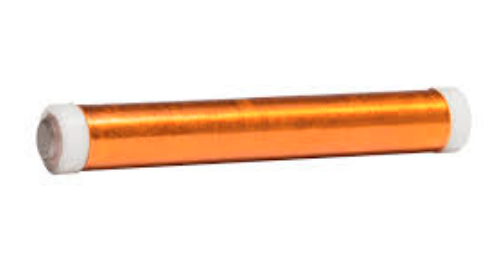
\includegraphics[height=40mm]{Figures/Magnetorquers}
  \end{center}
  \caption{Example Magnetorquer\cite{qp16}}
\end{figure}

An example of magnetorquer effectiveness is its ability to detumble
during an orbit, and how many orbits it will take to completely
detumble the spacecraft. First, the magnetorquer will have a magnetic
moment value associated with the physical parameters of the rod
$\mu$. First the average torque is computed by taking the magnetic
moment and multiplying it with the average field strength and the
point (from IGRF model). Then, this average torque is multiplied by
total time of the orbit $T_p$ to determine 
the magnetorquer’s momentum effectiveness over one orbit. Note that
the torque from the magnetorquer’s $\vec{M}_{MT}$ is substracted by
the total disturbance torques $\vec{M}_D$ to obtain the total
effectiveness of the magnetorquers. From this, it is possible to
calculate the number of orbits it will take to detumble the spacecraft
on an axis.  

\begin{equation}
  N_{orbits} = \frac{||\vec{H_S}||}{T_p(\vec{M}_{MT}-\vec{M}_D)}
\end{equation}

The magnetorquer effectiveness boils down to the difference in the
total moment that the magnetorquers can produce and the total
disturbance momentum during the orbit. Then, the number of orbits that
it will take for the spacecraft to detumble in an axis is a function
of the magnetorquer effectiveness divided by the initial angular
momentum in each axis.

\subsubsection{Reaction Wheels}

Reaction wheels are mechanical disks, or flywheels, that rotate the
satellite during orbit. The reaction wheels take in electrical power
and provide a torque to the satellite\cite{qp18}. This electrical power is
provided to a DC motor which then spins the reaction wheel. Because
momentum must be conserved, angular momentum must also be
conserved. Thus, by Newton’s third law, when the reaction wheel
rotates one direction the satellite rotates in the other. So, a
minimum of one reaction wheel is placed on each axis to control the
rotation in all directions. The primary role of a reaction wheel is to
point the satellite without the use of any fuel.
\begin{figure}[H]
  \begin{center}
  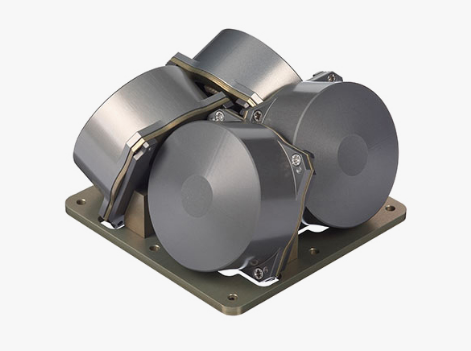
\includegraphics[height=40mm]{Figures/ReactionWheels}
  \end{center}
  \caption{Example Reaction Wheels\cite{qp19}}
\end{figure}

The inertia storage for reaction wheels is a parameter that can be
used to seek out the best reaction wheels for the spacecraft. Once the
inertia storage is computed, one can search for reaction wheels with
the proper amount of inertia storage required. For example, if a
reaction wheel with an inertia storage of 50 mNms is needed, one can
go to Blue Canyon Technologies website to find the datasheets for
their different reaction wheels. From there, it can be determined that
the best fit would be the RWP050 reaction wheels\cite{qp20}.

Once an estimate of the inertia of the satellite is obtained, they can
be used to compute the required inertia storage of the reaction wheels. The 
tip off rate for a spacecraft is the rate at which the spacecraft’s
angular velocity is altered due to its deployment. The following
equation shows how momentum can be calculated due to tip off.

\begin{equation}
||\vec{H}_S|| = max({\bf I}_S)\omega_{TOR}f
\end{equation}
where $\omega_{TOR}$ is typically set at 10 deg/s and f the factor of
safety is typically set to 2.

\subsubsection{Thrust Vector Control (TVC)}

When aerodynamic control surfaces are ineffective, TVC is a solution
to maintain the vehicle's correct attitude for the thrust duration. It
accomplishes this goal by gimballing (rotating) the thrust chamber or
by redirecting the exhaust-gas flow to develop torque \cite{qp21}. However,
thrust vectoring only moves the vehicle in two directions. TVC is
typically used to control pitch and yaw attitude on boosters and upper
stages.
\begin{figure}[H]
  \begin{center}
  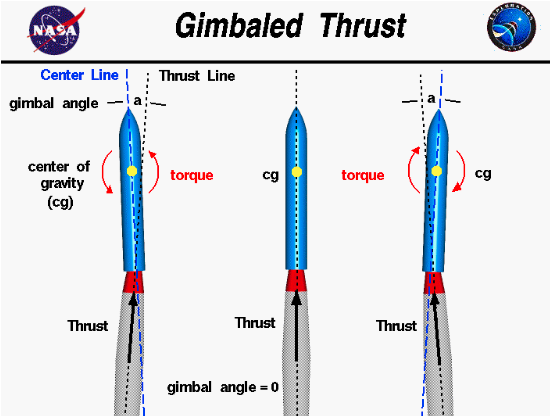
\includegraphics[height=70mm]{Figures/TVS}
  \end{center}
  \caption{TVC Diagram\cite{qp22}}
\end{figure}
%\subsubsection{Pointing Analysis}

\subsubsection{Reaction Control System (RCS)}

Reaction control systems are small thrusters. These thrusters alter
the speed of the spacecraft's rotational or spinning motion. They are
good for making quick turns and are used for getting to new
orientations quickly. Reaction control thrusters are typically in
"couples" or pairs of thrusters that together can spin the spacecraft
without changing the lateral velocity. In addition, these thrusters
usually work great with reaction wheels. When reaction wheels slow
down, they produce a force. The RCS will oppose this force which
allows the spacecraft to remain in the intended
orientation\cite{qp23}.
\begin{figure}[H]
  \begin{center}
  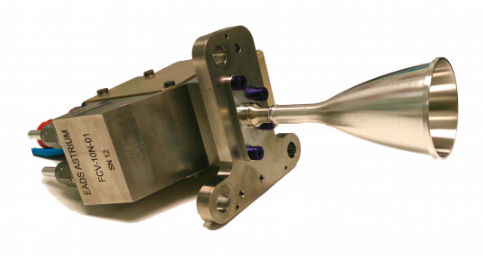
\includegraphics[height=50mm]{Figures/RCS}
  \end{center}
  \caption{Example RCS Thruster \cite{qp24}}
\end{figure}

\subsubsection{Control Moment Gyro}

A CMG is a spinning rotor at a constant speed [25]. Similar to a
reaction wheel, a CMG also has a spinning fly-wheel controlled by a
brushless motor. However, the spin axis of a CMG can rotate with the
help of a second motor placed on a gimbal axis. If the angular
momentum can only rotate in a fixed plane, it is known as a single
gimbal control moment gyros (SGCMG). GMCS are usually more efficient
and produce higher torque than reaction wheels as the size of the unit
increases\cite{qp26}.
\begin{figure}[H]
  \begin{center}
  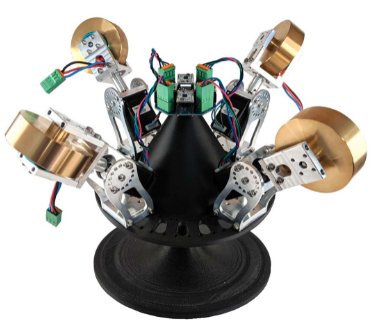
\includegraphics[height=50mm]{Figures/CMG}
  \end{center}
  \caption{Example CMG \cite{qp27}}
\end{figure}

\subsection{Spacecraft Attitude Determination}

Attitude determination is a fundamental portion of the ADACS board and
requires the vehicle to determine it's orientation with respect to an
inertial frame. The sections that follow detail the sensors and
fundamental attitude determination algorithms derived thus far. 

\subsubsection{Sensor Overview}

There are a multitude of sensors that are typically used on board
small sats. Note that most satellites use a combination of these
sensors rather than using all of them on one single satellite.

\begin{enumerate}[itemsep=-5pt]
  \item {\bf Magnetometers:} Only used in LEO, they measure the
    magnetic field in the body frame $\vec{\beta}_B = [\beta_x,\beta_y,\beta_z]^T$.
    \item {\bf Rate Gyros:} These sensors measure the angular velocity
      of the spacecraft in the body frame $p,q,r$.
    \item {\bf Solar Sensors:} These sensors can be coarse analog
      sensors with an accuracy of 45 degrees or can be high precision
      digital sensors that have accuracy down to 1 degree. Sun senors
      return an azimuth $\upsilon$ and declination $\delta$ angle which can be then
      translated into a vector in the body frame $\vec{S}_B$.
    \item {\bf Horizon Sensors:} Horizon sensors are typically used in
      LEO as they find the horizon of the Earth and use that for
      orientation information. These sensors also return an azimuth
      and declination angle that can be translated into a body frame
      vector $\vec{H}_B$.
      \item {\bf Startrackers:} Startrackers utilize a large aperture
        digital camera to photograph a starmap within the field of
        view of the lens. The photographed stars are then cross
        referenced with a starmap database and return the full
        quaternion vector.
\end{enumerate}

Some issues arise with all of these sensors. For example,
magnetometers must be activated when magnetorquers are turned off
otherwise those artificial magnetic fields will pollute the data. Rate
gyros are prone to drift while solar sensors can be quite
inaccurate. Startrackers also run the risk of being blinded by the Sun
and/or the Moon thus it is possible to design an
attitude determination algorithm that utilizes the Sun's ephemeris data
along with the Moon's ephemeris data in the event that the startracker
is obscured by the Sun/Moon.

\subsubsection{StarTracker}

A star tracker is another critical component of attitude control. This
device is a camera that points out from one face of the satellite. The
camera is able to detect the stars in its field of view (FOV) and
determine the location of the satellite based on this. Specifically,
the star tracker images the “starscape” to identify the known planets
and stars, and compares the imaged locations to the known locations
using the SPICE Toolkit\cite{qp28}. NASA Jet Propulsion Laboratory (JPL) has
produced the SPICE Toolkit for knowledge of the location of the
planetary bodies and stars and specific times\cite{qp29}.
\begin{figure}[H]
  \begin{center}
  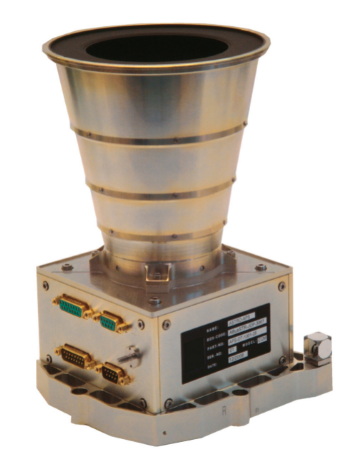
\includegraphics[height=50mm]{Figures/StarTracker}
  \end{center}
  \caption{Example StarTracker \cite{qp30}}
\end{figure}

\subsubsection{Sun Sensors}

A sun sensor is a device that senses the sun’s direction to measure
the position of the sun with respect to the sensor’s position. There
are three types of sun sensors. The first one is an analog sensor
whose output signal is a continuous function of the Sun angle. Next is
a sun presence sensor which provides a constant output signal when it
senses the sunlight. The last one is a digital sensor that produces
encoded discrete output that is measured by the sun angle function.

Sun sensors work based on the entry of light into a thin slit on top
of a rectangular chamber with the bottom part lined with a group of
light-sensitive cells. The chamber casts an image of a thin line on
the chamber bottom. The cells at the bottom of the rectangular chamber
measure the distance of the image and the refraction angle by using
the chamber height. The cells convert the incoming photons into
electrons and develop voltages which are converted into digital
signals. the direction of the sun can be computed when the sensors are
perpendicular to each other \cite{qp31}.
\begin{figure}[H]
  \begin{center}
  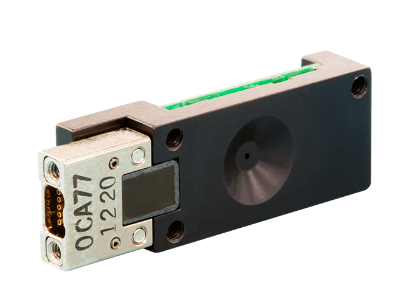
\includegraphics[height=50mm]{Figures/SunSensor}
  \end{center}
  \caption{Example Sun Sensor \cite{qp32}}
\end{figure}

\subsubsection{Horizon Sensor}

The horizon sensor is a sensor used by spacecraft in LEO to determine
the location of the Earth’s horizon. There are two main types of
horizon sensors: statics and scanning. A static horizon sensor is able
to detect the infrared radiation emitting from the Earth’s surface to
locate the horizon of Earth. Scanning horizon sensors are much more
complicated and use a system consisting of a spinning mirror to direct
light onto a bolometer. This bolometer can sense when the infrared
signal is present or lost. So, as the mirror rotates and reflects
infrared light into the bolometer, the bolometer is able to detect
when the signal is present or lost to determine the edge of the
horizon\cite{qp37}.  
\begin{figure}[H]
  \begin{center}
  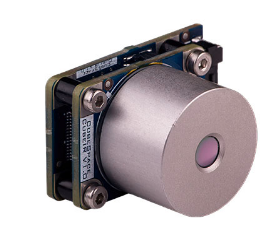
\includegraphics[height=50mm]{Figures/HorizonSensor}
  \end{center}
  \caption{Example Horizon Sensor \cite{qp1}}
\end{figure}

\subsubsection{Deep Space}

As explained earlier, in deep space it is possible to obtain a vector
to the Moon to be used in the attitude determination algorithm. The
Moon sensor would give a vector to the Moon in the body frame
$\vec{M}_B$ while an inertial vector would be needed $\vec{M}_I$. This
inertial Moon vector could be obtained via the Moon's
ephemeris data which could be loaded onto the satellite's processor
and use the orbital elements of the Moon to determine its position
relative to the Earth. However, the Moon's ephemeris data would more
than likely give the Moon's position relative to the Earth
($\vec{r}_{\Earth \rightarrow \Moon}$). The vector $\vec{M}_I$ would
then be given by
\begin{equation}
  \vec{M}_I = \vec{r}_{\Earth \rightarrow \Moon} - \vec{r}_{B}
\end{equation}
where $\vec{r}_B$ is the satellite's position relative to the
Earth. Note however that the position of the satellite relative to the
Earth would need to be obtained via the Deep Space Network (DSN) and a
combination of state estimation by integrating the orbital
equations. The reference paper \cite{Munoz} is a great paper that
details all the different kinds of sensors and their algorithms. This
section will eventually be supplemented by the material in that
reference paper.

\subsection{Position Estimation}

Position estimation is for determining the placement or location of
the spacecraft in orbit. This can often be confused with attitude
estimation, however, this can be clarified with an analogy. A human's
posture is their attitude while their location, or place in reference
to something else, is their position. This analogy can be transferred
to spacecraft attitude and position. Position estimation is how
mission control determines the location of the spacecraft in space. It
is vital for the spacecraft to know its position in order for the on
board sensors to work as intended. Position estimation is similar to
attitude control in the sense that the orbit plays a large role in
determining the proper component. The major options for attitude
estimation are Global Positioning Systems and the Ground Station
Network. 

\subsection{Trade Studies}

Tradeoffs and considerations are analysis tools used to compare
different components. It is not always obvious which component is best
for a subsystem function. As shown in the previous sections, there are several
options for attitude control, attitude estimation, and position
estimation. It may not stand out at first glance which components are
the best, so it is up to the team to perform a proper tradeoff
analysis, a.k.a a trade study. What this typically looks like is a
comparison of the different parameters of the components. For example,
if the GNC team decides to look at an integrated system for attitude
estimation, a trade study can be conducted to compare the mass, power,
volume, and momentum storage for different Blue Canyon Technologies
XACT systems \cite{qp20}. It is important to keep this trade study organized
and regularly updated, so it is recommended that a table is created to
compare these parameters.  

The name “tradeoff” comes from the fact that for a system it is
typical that one feature must be compromised for the other. For
example, to get more power, it is probably reasonable to assume that
volume will be compromised because the size of the component will need
to increase to fit a larger power supply. Another example may be that
in order to increase the volume of a component to fit a larger
payload, the mass will be compromised and may increase. These
compromises especially become issues when they interfere with the
subsystem requirements.

\subsection{Risks}

Risk assessments are arguably the most important task for the GNC
team. It is crucial that the entire system is taken into consideration
and assessed for possible failures because only one part needs to fail
to cripple the whole mission. This includes non physical issues such
as increased lead times on parts for example. The purpose of a risk
assessment is to identify all possible risks, their severity and
likelihood and to come up with mitigation strategies for those risks. 

The purpose of risk assessments is to determine mitigation strategies
so that the identified risks may be prevented. These mitigations are
discussed amongst the team and heavily considered while designing the
subsystem. Mitigation strategies can range anywhere from simply
creating a preflight checklist to diverting control from one component
to another in the event of a failure. These strategies are the main
purpose of creating a risk analysis in the first place, so careful
deliberation should be used when creating them. 

The best way to conduct a risk assessment is by creating a risk table
for the GNC subsystem. A risk table will list out the possible risks
determined by the team and their subsequent mitigation strategies. It
will also list out the likelihood and severity of each individual risk
as decided by the team. These can be determined in any way deemed
reasonable by the team, but is most often used on a scale of one to
five for each category. These values can then be input into a risk
criticality matrix which shows which risks are of the greatest threat
level.  

It is important that risk statements are written in a specific way to
avoid any confusion or miscommunication between the different
subteams. A risk statement consists of four parts: the condition,
departure, asset and consequence. The condition is a single phrase
that describes the current key fact-based situation or environment
that is causing concern, doubt, anxiety, or uneasiness. The departure
describes a possible change from the design or plan. It is an
undesired event that is made credible or more likely as a result of
the condition. The asset is an element of the system or plan. It
represents the primary resource that is affected by the individual
risk. The consequence is a single phrase that describes the
foreseeable, credible negative impact(s) to meet performance
requirements. A proper risk statement should utilize these four parts
in a format similar to the following: “Given that [CONDITION], there
is a possibility of [DEPARTURE] adversely impacting [ASSET], which can
result in [CONSEQUENCE]”

\subsection{Conclusions}

The GNC subsystem's purpose is to know where the spacecraft is, where
it needs to go, and determine how it will get there. These
requirements are determined by the overall mission goal of the
spacecraft. The system constraints are divided into three main
categories: the attitude control, attitude estimation, and position
estimation. The attitude control is how the spacecraft will maintain
its current orientation during orbit. Magnetorquers, reaction wheels,
thrust vector control, reaction control systems, and control moment
gyros are all common components used to counteract the disturbance
torques and maintain the desired orientation. Attitude estimation is
how the spacecraft estimates its current orientation. This is commonly
achieved by star trackers, sun sensors, magnetometers, rate gyros,
accelerometers, and horizon sensors. Lastly, the position estimation
is knowing the precise location of the satellite during its orbit. GPS
and the GSN are the two most common methods for determining the
satellites position.  

Not only are the components important but one must also consider the
trade-offs and risks associated with the mission. Risks must be
assessed and properly mitigated in order to ensure the safety and
success of the spacecraft. This is done by creating risk tables using
if-then terminology.
